\documentclass[tikz]{standalone}
\usepackage{tikz}
\usetikzlibrary{patterns,snakes}
 
\begin{document}
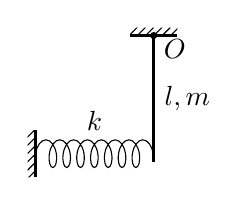
\begin{tikzpicture}
	\draw [very thick] (2,0) -- (2,-1.6) node [midway, right] {$l, m$};
	\draw [snake=coil, segment amplitude=5pt, segment length=5pt] (0.5,-1.5) -- (2, -1.5) node [midway, above=5pt] {$k$};
	\draw [thick] (0.5,-1.8)--(0.5,-1.2) (1.7,0)--(2.3,0);
	\draw [draw=none, pattern=north east lines] (0.4,-1.8) rectangle (0.5,-1.2) 
											   (1.7,0) rectangle (2.3,0.1);
	\draw [thick, fill] (2, 0) circle (0.03) node [below=5pt,right] {$O$};
\end{tikzpicture}
\end{document}